\documentclass[11pt,a4paper]{article}
\usepackage[left=25mm,right=15mm,top=15mm,bottom=15mm]{geometry}
\usepackage[utf8x]{inputenc}
\usepackage[L7x]{fontenc}
\usepackage[lithuanian]{babel}
\usepackage{url}
\usepackage{float}
\usepackage{graphicx}

\title{Moderniosios operacinės sistemos\\Namų darbas 1\\Variantas 1}
\author{Maksim Norkin\\ AKSfm-15}

\begin{document}

    \maketitle

    \section{Užduotis}

    Operandą 11, esantį atminties ląstelėje adresu $700$, sudėti su operandu 4, esančiu 5-me Į-I buferyje. Rezultatą išsaugoti atminties ląstelėje adresu $710$.

    \begin{figure}[H]
        \centering
        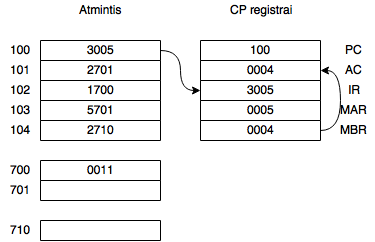
\includegraphics[width=200px]{img/operacines-sistemos-01.png}
        \caption{Programa pradedama vykdyti adresu $100$. Į IR yra pakraunamas operacijos kodas ir Į-I adresas, kuris yra perduodamas į atminties adreso registrą. Atminties buferio registras gauna iš išorinės atminties adreso reikšmę. Ta reikšmė toliau nukeliauja į akumuliatorių.}
    \end{figure}

    \begin{figure}[H]
        \centering
        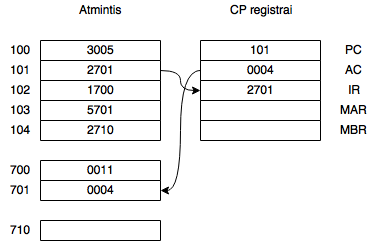
\includegraphics[width=200px]{img/operacines-sistemos-02.png}
        \caption{Tolimesnė eiga yra išsaugoti nuskaitytą vertę iš Į-I į vietinę atmintį. Tai yra pasiekiama su $2$ operando kodu nurodant norimą vietą, kur išsaugoti skaičių iš akumuliatoriaus. Šiuo atveju skaičius yra saugomas $701$ atminties ląstelėje.}
    \end{figure}

    \begin{figure}[H]
        \centering
        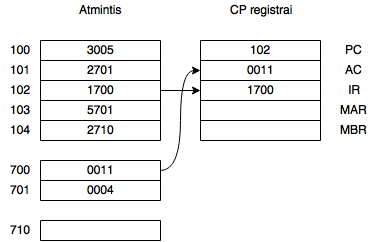
\includegraphics[width=200px]{img/operacines-sistemos-03.png}
        \caption{Dabar galime pradėti vykdyti sumavimo užduotį, pirmiausiai pasikrovę skaičių iš $700$ atminties į akumuliatoriaus registrą.}
    \end{figure}

    \begin{figure}[H]
        \centering
        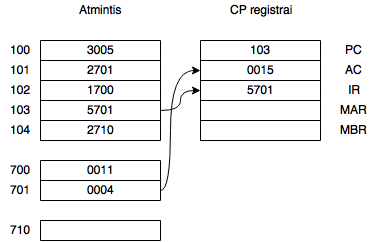
\includegraphics[width=200px]{img/operacines-sistemos-04.png}
        \caption{Esantį akumuliatoriuje skaičių galima sudėti su atminties bloke esančiu skaičiumi.}
    \end{figure}

    \begin{figure}[H]
        \centering
        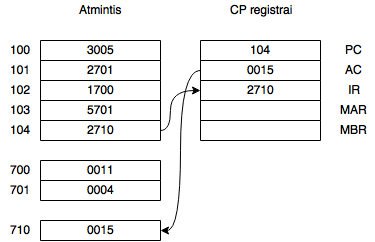
\includegraphics[width=200px]{img/operacines-sistemos-05.png}
        \caption{Turimą skaičių įrašome į atmintį ir baigiame darbą.}
    \end{figure}

    \section{Išvados}

    Darbo metu buvo patiekta programos vykdymo diagrama su $PC$, $AC$, $IR$, $MAR$ ir $MBR$ registrais ir atminties blokine schema.

\end{document}